\documentclass[14pt,a4paper,report]{report}
\usepackage[a4paper, mag=1000, left=2.5cm, right=1cm, top=2cm, bottom=2cm, headsep=0.7cm, footskip=1cm]{geometry}
\usepackage[utf8]{inputenc}
\usepackage[english,russian]{babel}
\usepackage{indentfirst}
\usepackage[dvipsnames]{xcolor}
\usepackage[colorlinks]{hyperref}
\usepackage{listings} 
\usepackage{fancyhdr}
\usepackage{caption}
\usepackage{amsmath}
\usepackage{graphicx}
\usepackage{amsmath}
\usepackage{booktabs}
\usepackage{array}
\newcolumntype{P}[1]{>{\centering\arraybackslash}p{#1}}
\hypersetup{
colorlinks = true,
linkcolor = black
}

\usepackage{titlesec}
\titleformat{\chapter}
{\Large\bfseries} % format
{} % label
{0pt} % sep
{\huge} % before-code


\DeclareCaptionFont{white}{\color{white}} 

% Listing description
\usepackage{listings} 
\DeclareCaptionFormat{listing}{\colorbox{gray}{\parbox{\textwidth}{#1#2#3}}}


\captionsetup[lstlisting]{format=listing,labelfont=white,textfont=white}
\lstset{ 
% Listing settings
inputencoding = utf8,	
extendedchars = \true, 
keepspaces = true, % Поддержка кириллицы и пробелов в комментариях
language = C, % Язык программирования (для подсветки)
basicstyle = \small\sffamily, % Размер и начертание шрифта для подсветки кода
keywordstyle=\color{blue}\ttfamily,
stringstyle=\color{red}\ttfamily,
commentstyle=\color{green}\ttfamily,
morecomment=[l][\color{magenta}]{\#},
numbers = left, % Где поставить нумерацию строк (слева\справа)
numberstyle = \tiny, % Размер шрифта для номеров строк
stepnumber = 1, % Размер шага между двумя номерами строк
numbersep = 5pt, % Как далеко отстоят номера строк от подсвечиваемого кода
backgroundcolor = \color{white}, % Цвет фона подсветки - используем \usepackage{color}
showspaces = false, % Показывать или нет пробелы специальными отступами
showstringspaces = false, % Показывать или нет пробелы в строках
showtabs = false, % Показывать или нет табуляцию в строках
frame = single, % Рисовать рамку вокруг кода
tabsize = 2, % Размер табуляции по умолчанию равен 2 пробелам
captionpos = t, % Позиция заголовка вверху [t] или внизу [b] 
breaklines = true, % Автоматически переносить строки (да\нет)
breakatwhitespace = false, % Переносить строки только если есть пробел
escapeinside = {\%*}{*)} % Если нужно добавить комментарии в коде
}

\begin{document}

\def\contentsname{Содержание}

% Titlepage
\begin{titlepage}
\begin{center}
\textsc{Санкт-Петербургский Политехнический 
Университет Петра Великого\\[5mm]
Кафедра компьютерных систем и программных технологий}

\vfill

\textbf{Отчёт по лабораторной работе №3\\[3mm]
на тему: «Методы сглаживания изображений»\\[3mm]
Курс: «Разработка графических приложений»\\[41mm]
}
\end{center}

\hfill
\begin{minipage}{.4\textwidth}
Выполнил студент:\\[2mm] 
Волкова М.Д.\\
Группа: 13541/2\\[5mm]

Проверил:\\[2mm] 
Абрамов Н.А.
\end{minipage}
\vfill
\begin{center}
Санкт-Петербург\\ \the\year\ г.
\end{center}
\end{titlepage}

% Contents
\tableofcontents
\clearpage

\chapter{Лабораторная работа №2}

\section{Цель работы}
Разработать программу на языке С для растеризации загруженной модели на экран

\section{Описание программы}
\begin{enumerate}
\item Возможности программы:

\begin{enumerate}
\item Загрузка трехмерной модели из OBJ-файла
\item Растеризация каркаса трехмерной модели
\item Обеспечение вращения камеры вокруг трехмерной модели
\end{enumerate}

\item Входные параметры программы:

\begin{enumerate}
\item Ширина и высота окна
\item Вертикальный угол обзора камеры для выполненя перспективной проекции
\item Ближняя и дальняя плоскости отсечения камеры
\item Дистанция от камеры до загруженной модели
\item Скорость вращения камеры вокруг модели (градус/сек)
\end{enumerate}

\item Выходные параметры программы:

\begin{enumerate}
\item Последовательность кадров, выводимая на экран
\end{enumerate}
\item Порядок работы программы:
\begin{enumerate}
\item Загрузка трехмерной модели в вершинные и индексные буфера
\item Определение центра модели (можно считать, что матрица мира для модели – единичная)
\item Формирование матрицы проекции
\item (Далее – для очередного кадра:)
\begin{enumerate}
\item Формирование матрицы вида исходя из координат центра модели, дистанции до модели и скорости вращения камеры
\item Преобразование вершин модели в экранные координаты 
\end{enumerate}
\end{enumerate}

\end{enumerate}
\clearpage

\section{Ход работы}
В дополнение к уже установленной ранее библиотеке OpenCV дополнительно была установлена библиотека GLM, предназначенная для работы с векторами и матрицами размерности до 4-х. Для работы с форматом OBJ использована библиотека TinyObj.

После загрузки, установки и настройки необходимых библиотек была составлена и протестирована нижеследующая программа.

\subsection{Настройка фиксированной камеры}
В OpenGL при использовании фиксированного конвейера есть ровно две матрицы, относящихся к трансформациям точек и объектов:
\begin{itemize}

\item GL PROJECTION моделирует ортографическое или перспективное преобразование от трёхмерной усечённой пирамиды (т.е. от области видимости камеры) к трёхмерному кубу с длиной ребра, равной 2 (т.е. к нормализованному пространству).
\item GL MODELVIEW сочетает в себе два преобразования: от локальных координат объекта к мировым координатам, а также от мировых координат к координатам камеры.
\end{itemize}

За рамками фиксированного конвейера можно использовать столько матриц, сколько захочется. 

\begin{itemize}
\item поведение камеры описывается как ортографическим или перспективным преобразованием, так и положением камеры в мировом пространстве, то есть для моделирования камеры нужны GL PROJECTION и GL MODELVIEW одновременно
\item c другой стороны, для трансформаций над телами —  вращение предмета с помощью умножения координат на матрицу — нужна матрица GL MODELVIEW.
\end{itemize}

Настроим матрицу GL PROJECTION один раз для перспективного преобразования, а матрицу GL MODELVIEW будем постоянно модифицировать, когда локальная система координат очередного объекта не совпадает с мировой системой координат.

Начнём настройку камеры с GL MODELVIEW: зададим матрицу так, как будто бы камера смотрит с позиции camera position на точку model center, при этом направление “вверх” камеры задаёт вектор glm::vec3(0, 1, 0):

\begin{lstlisting}
camera = glm::lookAt(
                camera_position,
                model_center,
                glm::vec3(0, 1, 0)
        );
\end{lstlisting}

Для перспективного преобразования достаточно создать матрицу с помощью функции glm::perspective. Она принимает на вход несколько  параметров преобразования: горизонтальный угол обзора камеры, соотношение ширины и высоты, а также две граничных координаты для отсечения слишком близких к камере и слишком далёких от камеры объектов. 

Эти параметры легко увидеть на следующей иллюстрации:

\begin{figure}[h!]
\center{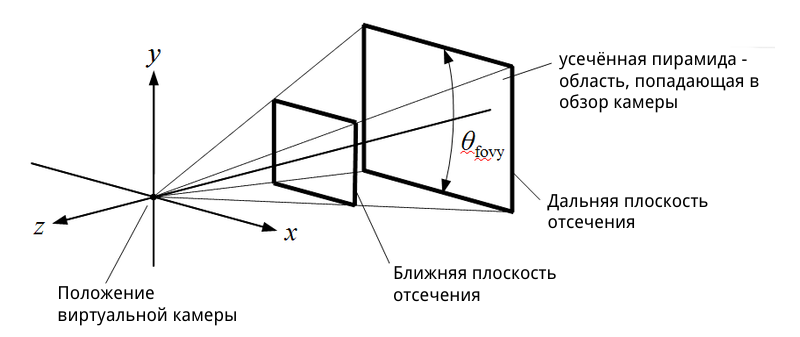
\includegraphics[width=0.8\linewidth]{images/perspective_volume.png}}
\label{ris:image}
\end{figure}

\clearpage
\begin{lstlisting}
projection = glm::perspective(
            glm::radians(fovy),
            screen_ratio,
            front,
            back)
\end{lstlisting}

\begin{itemize}
\item glm::radians(fovy) - Вертикальное поле зрения в радианах.

\item screen ratio - Отношение сторон.

\item front - Ближняя плоскость отсечения.

\item back - Дальняя плоскость отсечения.

\end{itemize}






\clearpage
\section{Результаты}
В качестве тестовой модели для проверки работоспособности программы использовалась модель чайничка, экспортированная стандартными средствами в формат OBJ.

 


\subsection{CvLineDrawer}
Параметры:

\begin{figure}[h!]
\center{\includegraphics[width=1\linewidth]{images/CvLineDrawer/options.png}}
\caption{Параметры}
\label{ris:image}
\end{figure}

Результат работы: 

\begin{figure}[h!]
\begin{minipage}[h]{0.47\linewidth}
\center{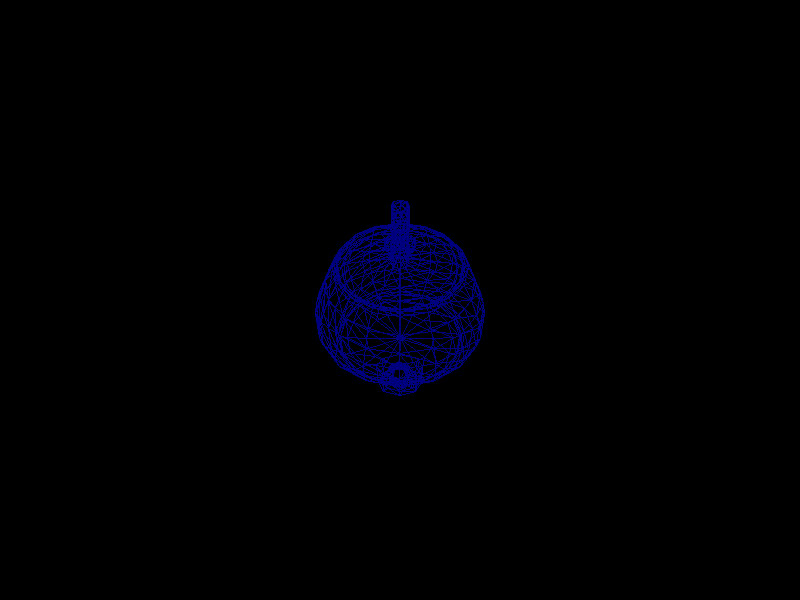
\includegraphics[width=1\linewidth]{images/CvLineDrawer/teapot0.png}} a) \\
\end{minipage}
\hfill
\begin{minipage}[h]{0.47\linewidth}
\center{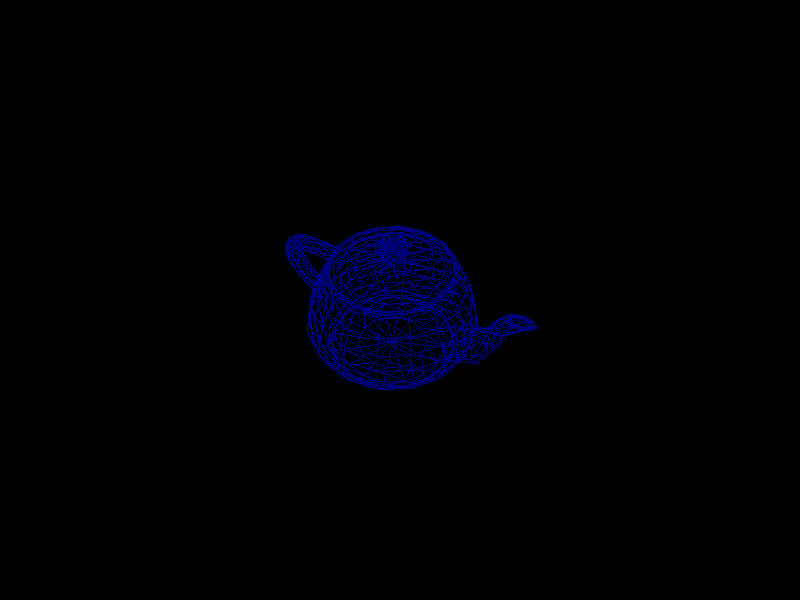
\includegraphics[width=1\linewidth]{images/CvLineDrawer/teapot1.png}} \\b)
\end{minipage}
\vfill
\begin{minipage}[h]{0.47\linewidth}
\center{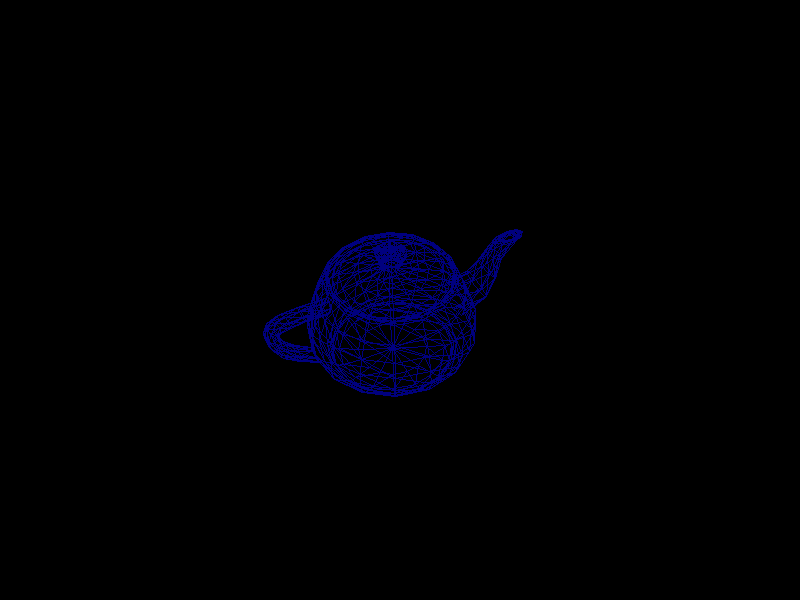
\includegraphics[width=1\linewidth]{images/CvLineDrawer/teapot2.png}} c) \\
\end{minipage}
\hfill
\begin{minipage}[h]{0.47\linewidth}
\center{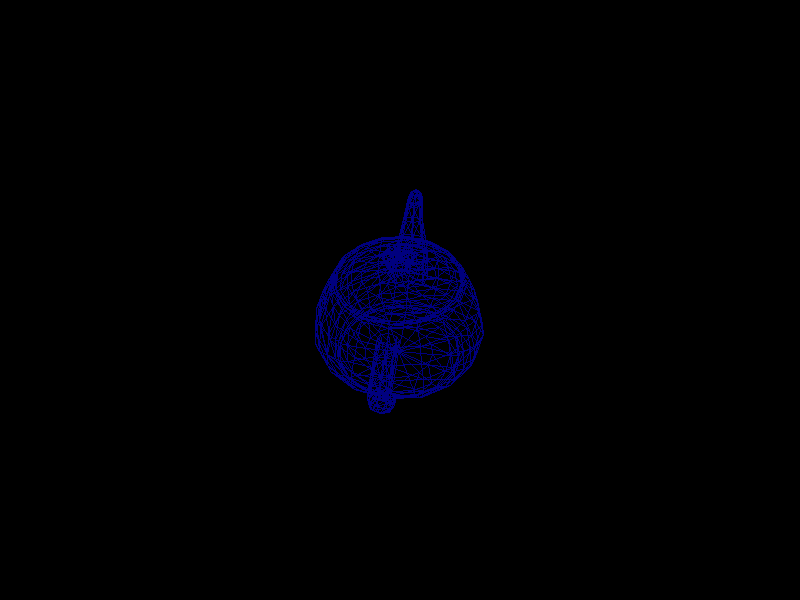
\includegraphics[width=1\linewidth]{images/CvLineDrawer/teapot3.png}} d) \\
\end{minipage}
\caption{Последовательно создаваемые изображения}
\label{ris:experimentalcorrelationsignals}
\end{figure}


\clearpage
\subsection{LineDrawer}
Параметры:

\begin{figure}[h!]
\center{\includegraphics[width=1\linewidth]{images/LineDrawer/options.png}}
\caption{Параметры}
\label{ris:image}
\end{figure}

Результат работы: 

\begin{figure}[h!]
\begin{minipage}[h]{0.47\linewidth}
\center{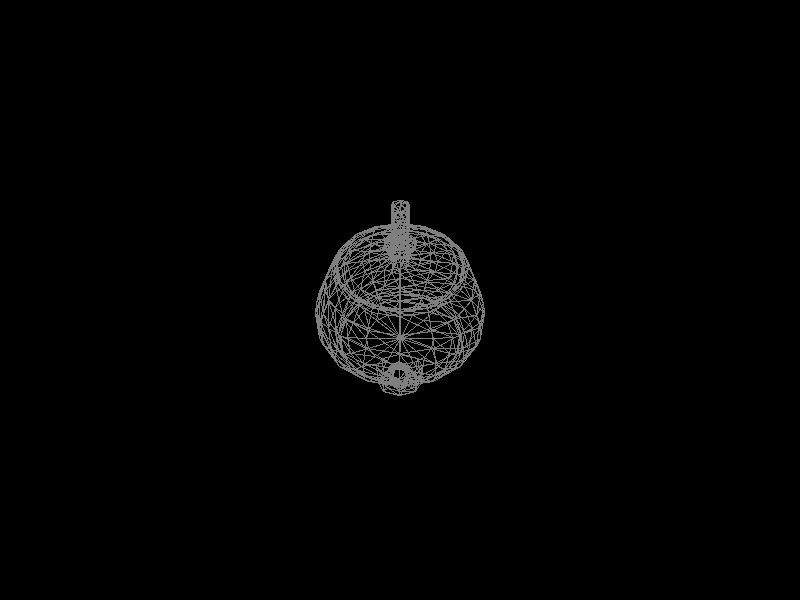
\includegraphics[width=1\linewidth]{images/LineDrawer/teapot0.png}} a) \\
\end{minipage}
\hfill
\begin{minipage}[h]{0.47\linewidth}
\center{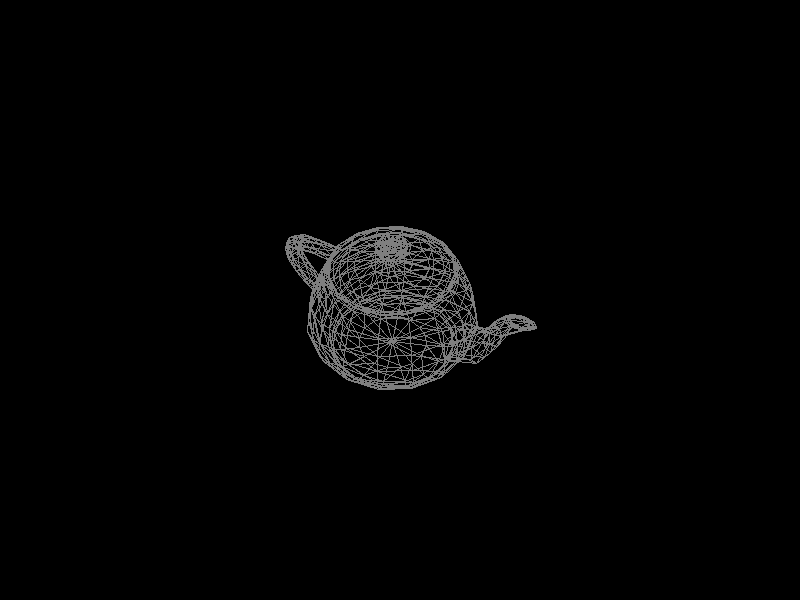
\includegraphics[width=1\linewidth]{images/LineDrawer/teapot1.png}} \\b)
\end{minipage}
\vfill
\begin{minipage}[h]{0.47\linewidth}
\center{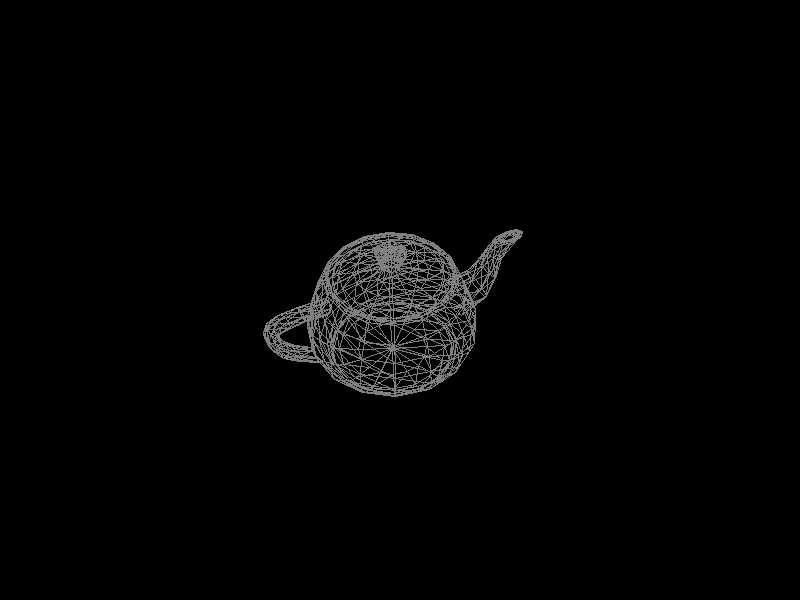
\includegraphics[width=1\linewidth]{images/LineDrawer/teapot2.png}} c) \\
\end{minipage}
\hfill
\begin{minipage}[h]{0.47\linewidth}
\center{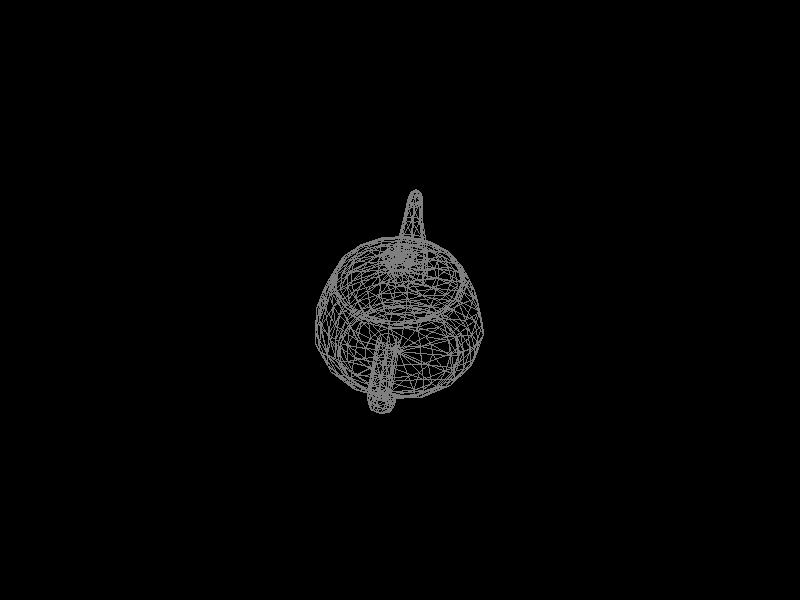
\includegraphics[width=1\linewidth]{images/LineDrawer/teapot3.png}} d) \\
\end{minipage}
\caption{Последовательно создаваемые изображения}
\label{ris:experimentalcorrelationsignals}
\end{figure}


\clearpage
\subsection{TriangleDrawer}
Параметры:

\begin{figure}[h!]
\center{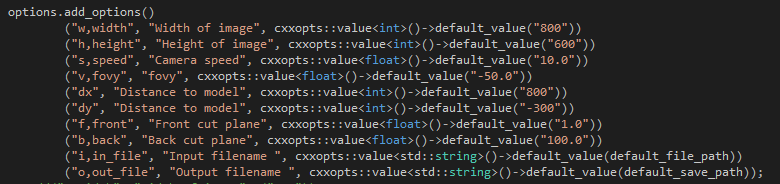
\includegraphics[width=1\linewidth]{images/TriangleDrawer/1/option.png}}
\caption{Параметры}
\label{ris:image}
\end{figure}

Результат работы: 

\begin{figure}[h!]
\begin{minipage}[h]{0.47\linewidth}
\center{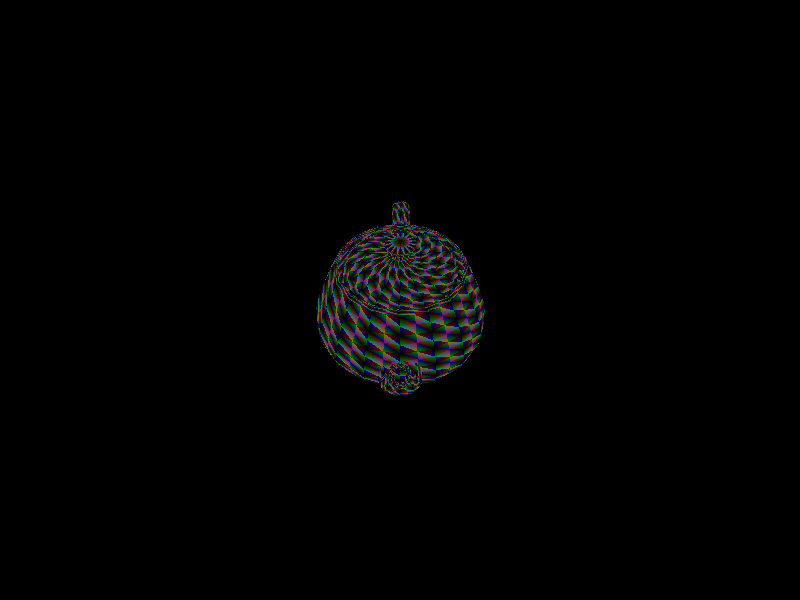
\includegraphics[width=1\linewidth]{images/TriangleDrawer/1/teapot0.png}} a) \\
\end{minipage}
\hfill
\begin{minipage}[h]{0.47\linewidth}
\center{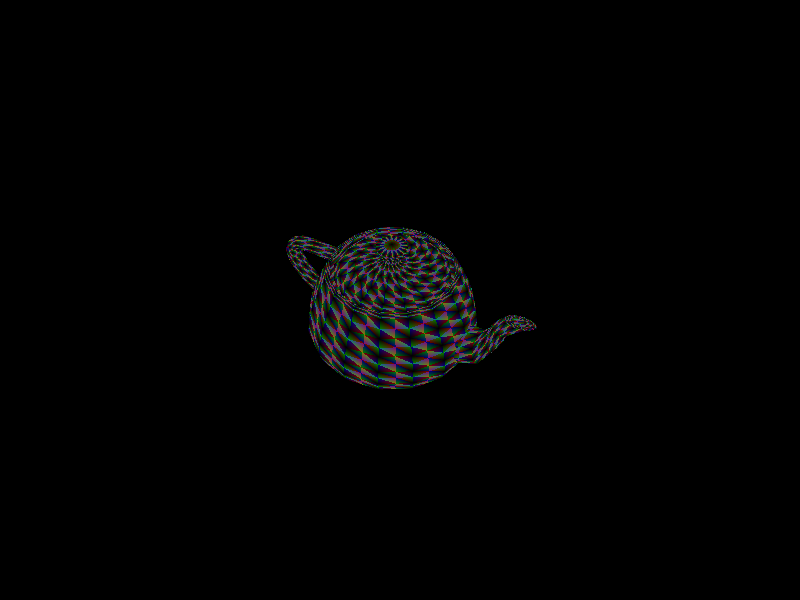
\includegraphics[width=1\linewidth]{images/TriangleDrawer/1/teapot1.png}} \\b)
\end{minipage}
\vfill
\begin{minipage}[h]{0.47\linewidth}
\center{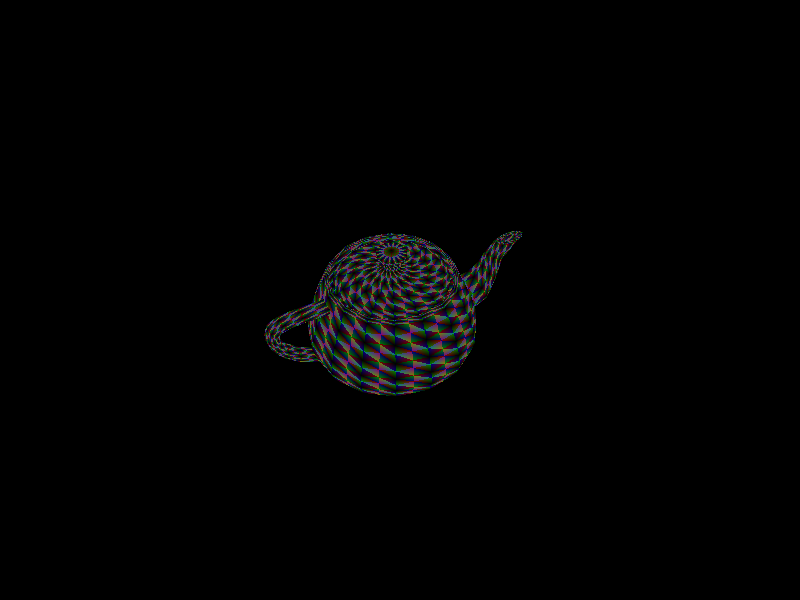
\includegraphics[width=1\linewidth]{images/TriangleDrawer/1/teapot2.png}} c) \\
\end{minipage}
\hfill
\begin{minipage}[h]{0.47\linewidth}
\center{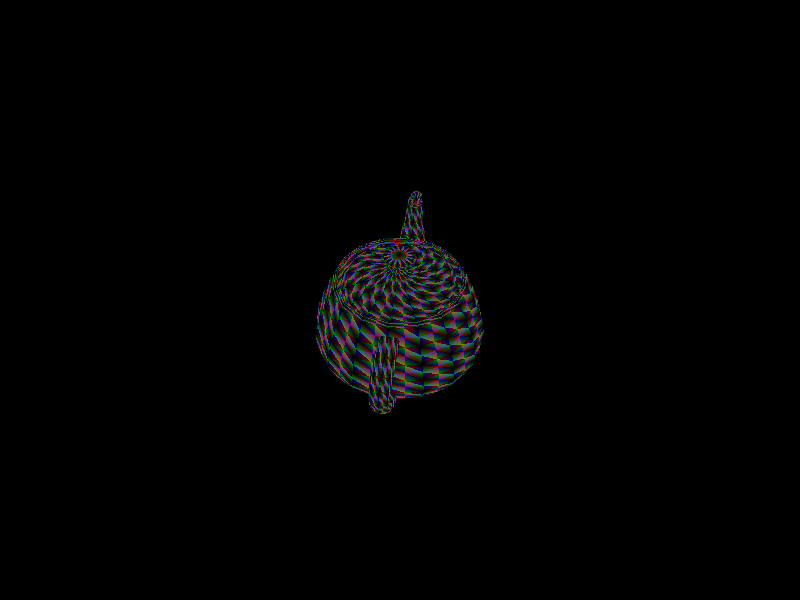
\includegraphics[width=1\linewidth]{images/TriangleDrawer/1/teapot3.png}} d) \\
\end{minipage}
\caption{Последовательно создаваемые изображения}
\label{ris:experimentalcorrelationsignals}
\end{figure}

Приведем еще несколько результатов, изменяя параметры камеры:

\clearpage
Параметры:

\begin{figure}[h!]
\center{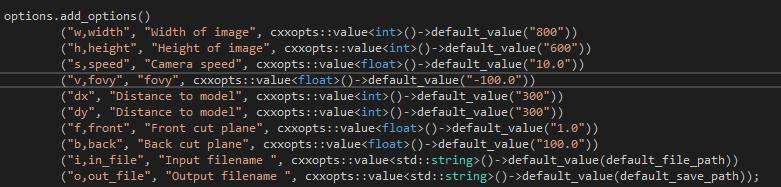
\includegraphics[width=1\linewidth]{images/TriangleDrawer/2/options.png}}
\caption{Параметры}
\label{ris:image}
\end{figure}

Результат работы: 

\begin{figure}[h!]
\begin{minipage}[h]{0.47\linewidth}
\center{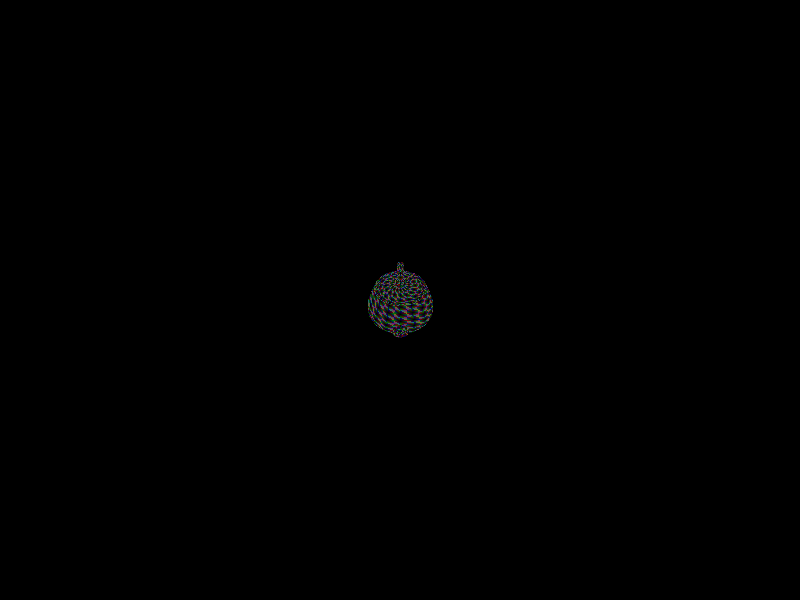
\includegraphics[width=1\linewidth]{images/TriangleDrawer/2/teapot0.png}} a) \\
\end{minipage}
\hfill
\begin{minipage}[h]{0.47\linewidth}
\center{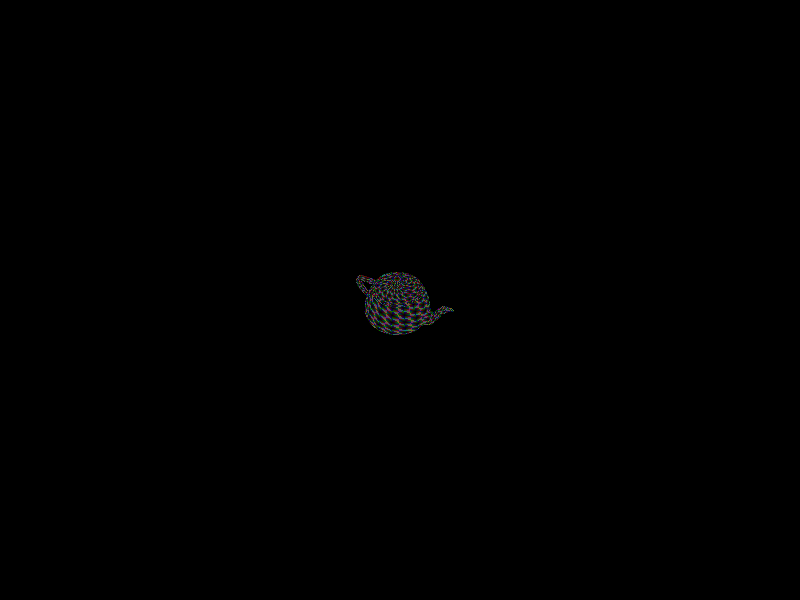
\includegraphics[width=1\linewidth]{images/TriangleDrawer/2/teapot1.png}} \\b)
\end{minipage}
\vfill
\begin{minipage}[h]{0.47\linewidth}
\center{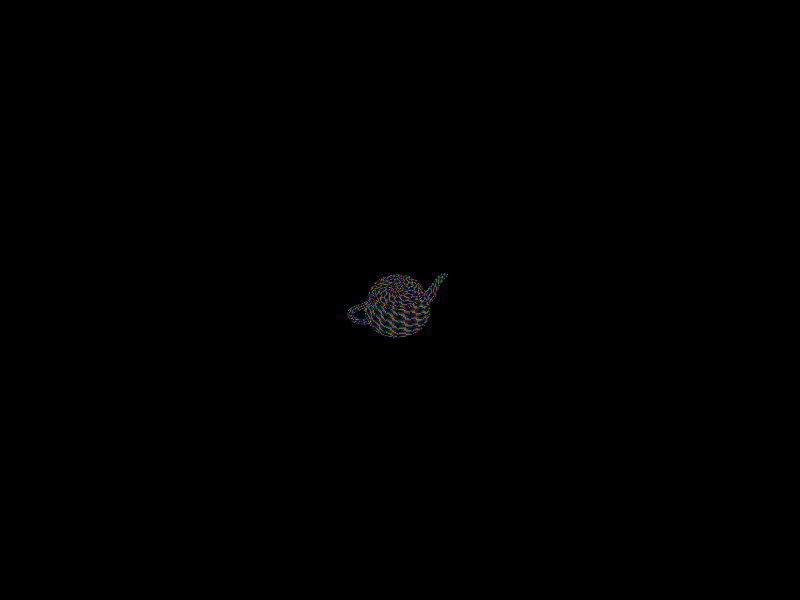
\includegraphics[width=1\linewidth]{images/TriangleDrawer/2/teapot2.png}} c) \\
\end{minipage}
\hfill
\begin{minipage}[h]{0.47\linewidth}
\center{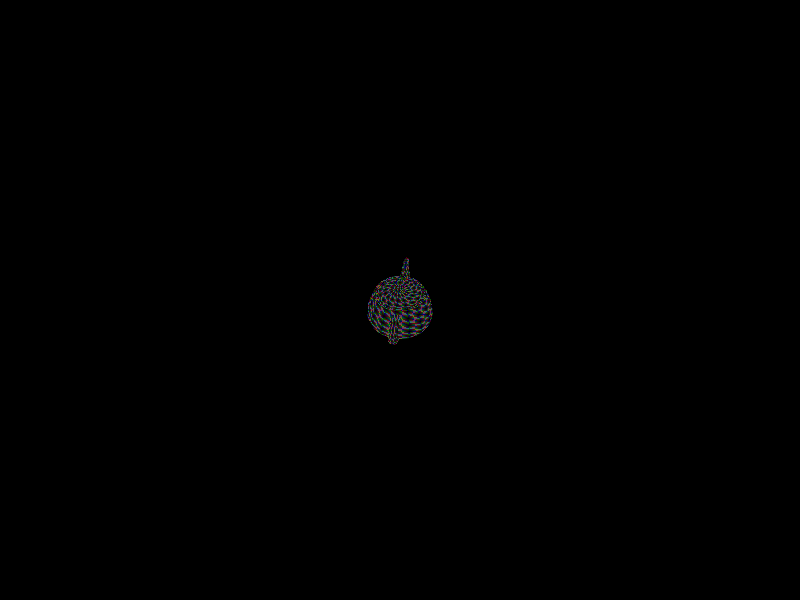
\includegraphics[width=1\linewidth]{images/TriangleDrawer/2/teapot3.png}} d) \\
\end{minipage}
\caption{Последовательно создаваемые изображения}
\label{ris:experimentalcorrelationsignals}
\end{figure}



\clearpage
Параметры:

\begin{figure}[h!]
\center{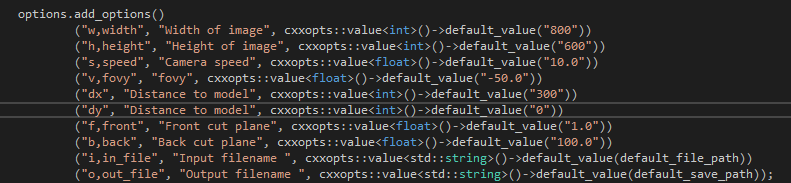
\includegraphics[width=1\linewidth]{images/TriangleDrawer/5/options.png}}
\caption{Параметры}
\label{ris:image}
\end{figure}

Результат работы: 

\begin{figure}[h!]
\begin{minipage}[h]{0.47\linewidth}
\center{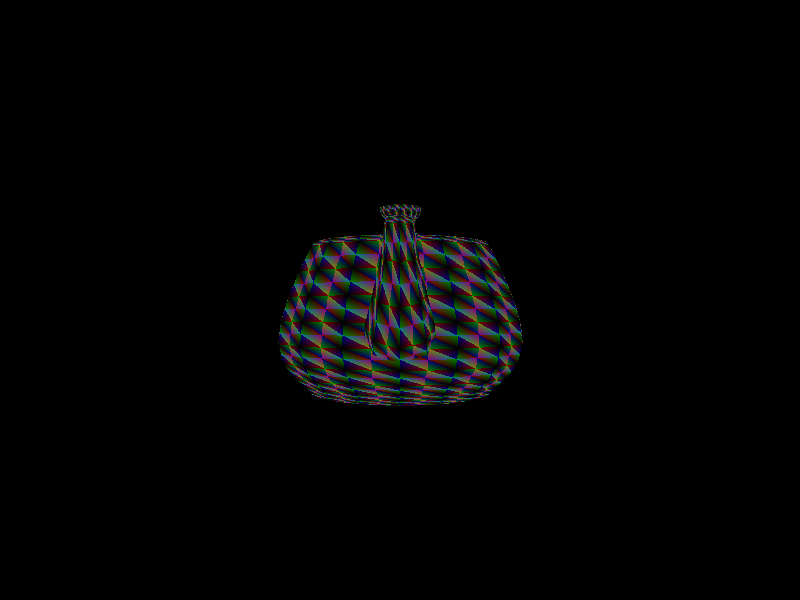
\includegraphics[width=1\linewidth]{images/TriangleDrawer/5/teapot0.png}} a) \\
\end{minipage}
\hfill
\begin{minipage}[h]{0.47\linewidth}
\center{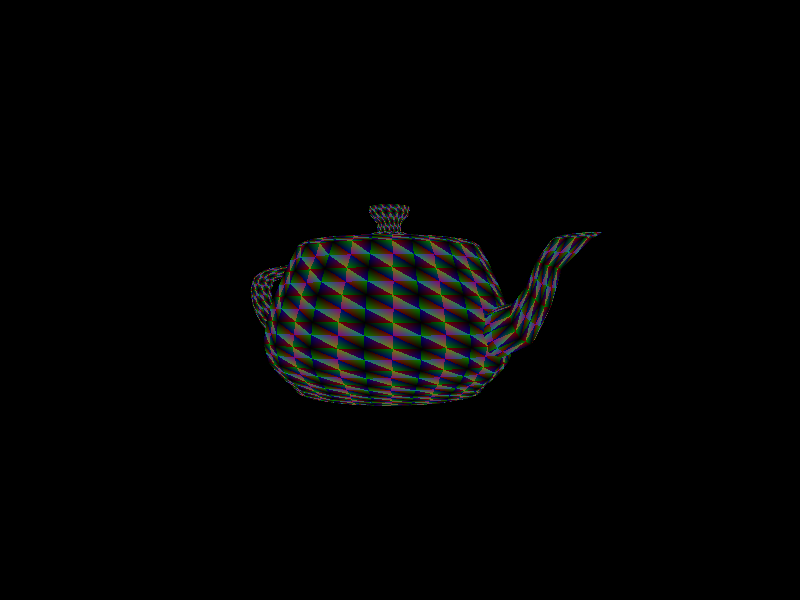
\includegraphics[width=1\linewidth]{images/TriangleDrawer/5/teapot1.png}} \\b)
\end{minipage}
\vfill
\begin{minipage}[h]{0.47\linewidth}
\center{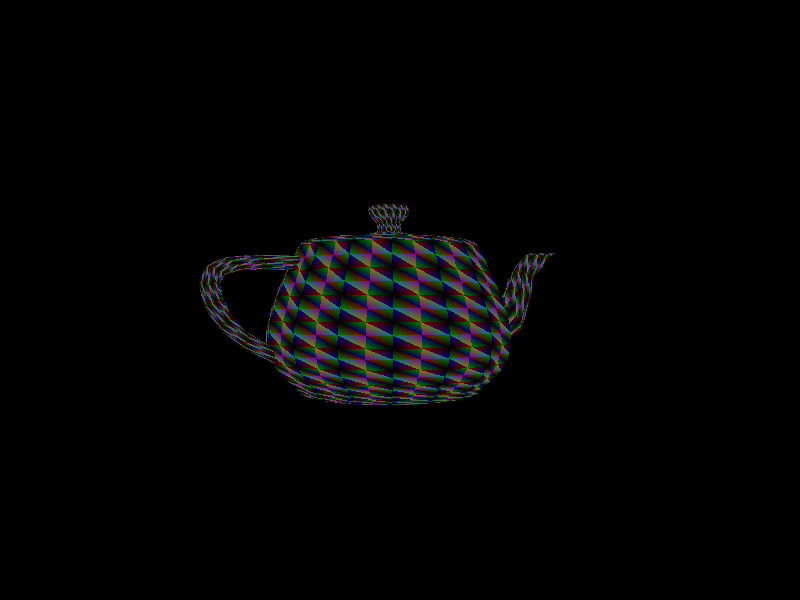
\includegraphics[width=1\linewidth]{images/TriangleDrawer/5/teapot2.png}} c) \\
\end{minipage}
\hfill
\begin{minipage}[h]{0.47\linewidth}
\center{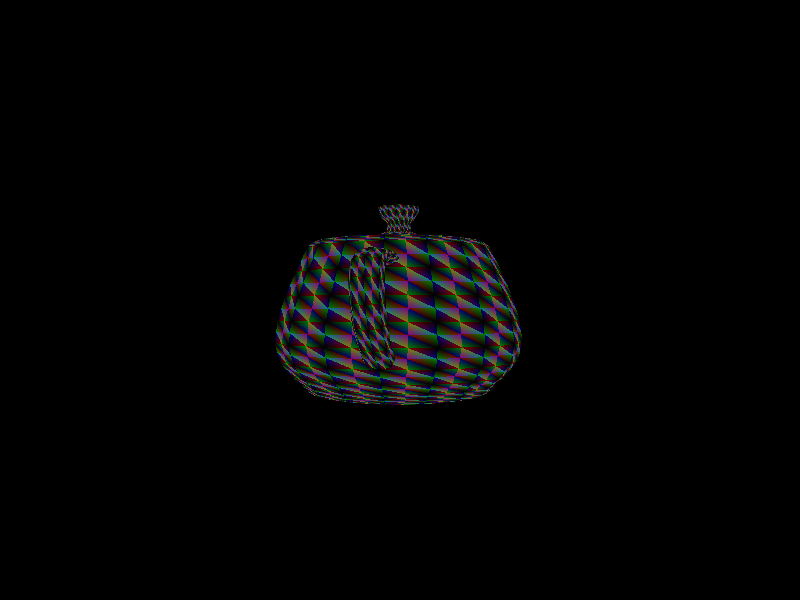
\includegraphics[width=1\linewidth]{images/TriangleDrawer/5/teapot3.png}} d) \\
\end{minipage}
\caption{Последовательно создаваемые изображения}
\label{ris:experimentalcorrelationsignals}
\end{figure}


\clearpage
Параметры:

\begin{figure}[h!]
\center{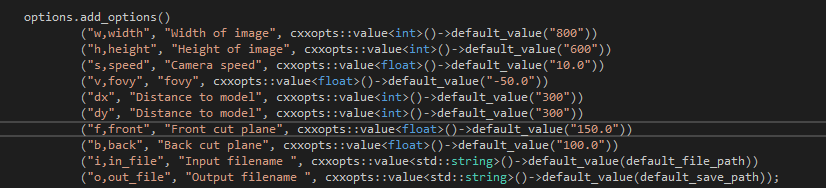
\includegraphics[width=1\linewidth]{images/TriangleDrawer/6/options.png}}
\caption{Параметры}
\label{ris:image}
\end{figure}

Результат работы: 

\begin{figure}[h!]
\begin{minipage}[h]{0.47\linewidth}
\center{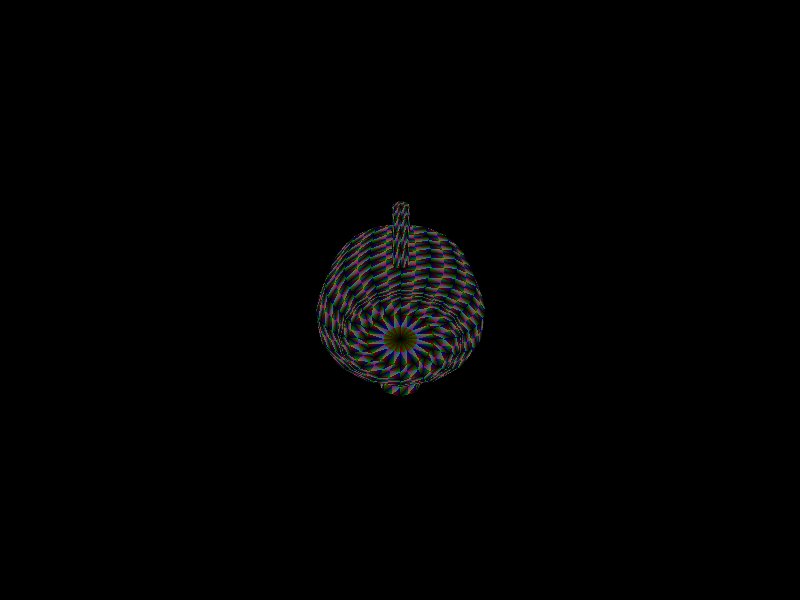
\includegraphics[width=1\linewidth]{images/TriangleDrawer/6/teapot0.png}} a) \\
\end{minipage}
\hfill
\begin{minipage}[h]{0.47\linewidth}
\center{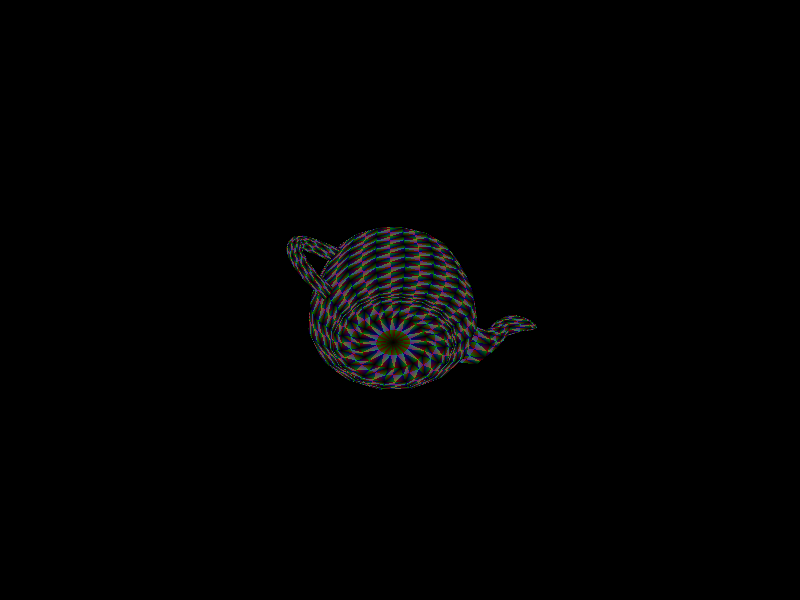
\includegraphics[width=1\linewidth]{images/TriangleDrawer/6/teapot1.png}} \\b)
\end{minipage}
\vfill
\begin{minipage}[h]{0.47\linewidth}
\center{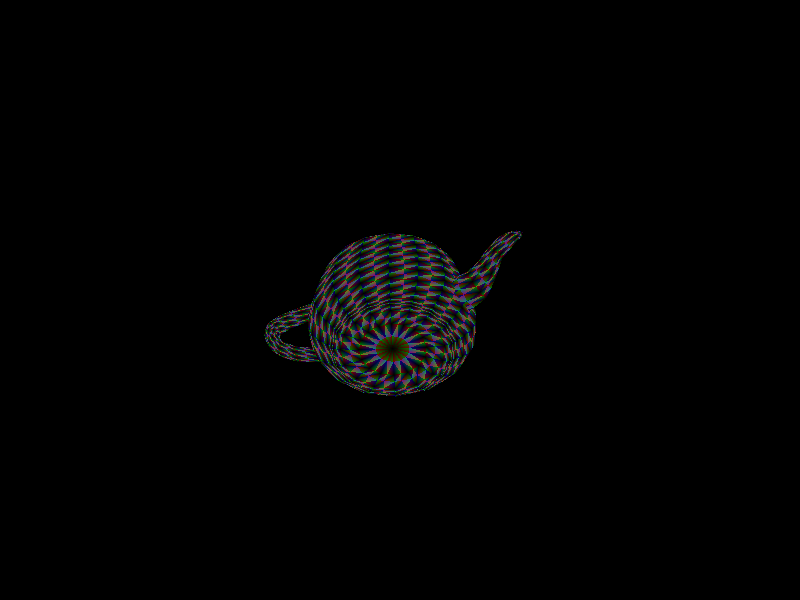
\includegraphics[width=1\linewidth]{images/TriangleDrawer/6/teapot2.png}} c) \\
\end{minipage}
\hfill
\begin{minipage}[h]{0.47\linewidth}
\center{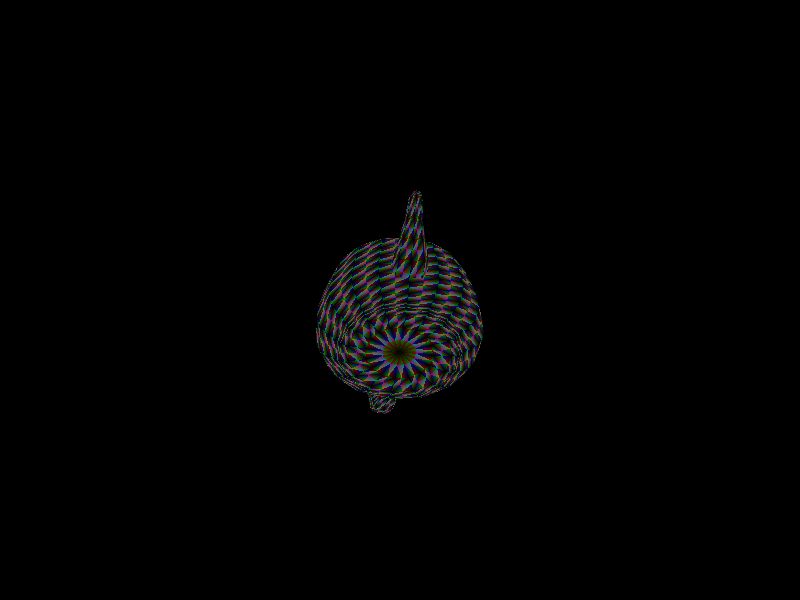
\includegraphics[width=1\linewidth]{images/TriangleDrawer/6/teapot3.png}} d) \\
\end{minipage}
\caption{Последовательно создаваемые изображения}
\label{ris:experimentalcorrelationsignals}
\end{figure}



Результатом работы стало двумерное анимированное изображение вращающегося каркаса выбранной ранее модели, которая в любой дискретный момент времени была повернута на некоторый угол вокруг мировых осей OX, OY, OZ.



\clearpage
\section{Вывод}
В данной работе была изучена библиотека GLM и составлена программа для визуализации трехмерной модели в виде проволочного каркаса с использованием средств библиотеки OpenCV.

Результаты визуализации отвечают ожиданиям при заданном смещении, повороте и масштабе модели. Для создания более полного представления наблюдателя о внешнем виде исходной модели, необходимо в дальнейшем реализовать отображение поверхностей модели, посредством треугольников, учитывая, что используемая библиотека TinyObj позволяет проводить разбиение произвольного полигона на треугольники автоматически при чтении файла модели.

\clearpage
\section{Листинг}
\lstinputlisting{listings/main.cpp}

\end{document}